\documentclass[12pt, aspectratio=169]{beamer} % aspectratio = either 43 or 169
\usepackage[utf8]{inputenc}
\usepackage{graphicx}
\usepackage[T1]{fontenc}
\graphicspath{ {./img/} }

\usetheme{Hannover}
\mode<presentation>


% title and author
\title{Presentación de la nueva estructura de guardias}
\author{Luis Palomero}

% document
\begin{document}

\frame{\titlepage}

\section{Introducción}


\begin{frame}{Overview}
\tableofcontents
\end{frame}

\begin{frame}{Problema}

  Se ha hecho necesaria la modificación de la estructura de guardias por que no se adapta a las necesidades actuales del proyecto.

  \begin{block}{Problemas identificados durante las guardias}
    \begin{itemize}
    \item No abarcan todo el período del fin de semana/festivo. Por ejemplo, si hay un error el viernes por la tarde, no se identifica
    \item Las guardias son \textit{de observación}. Si se identifican bugs en producción, según quién haga la guardia no se pueden resolver.
    \end{itemize}

    En caso de los bugs en producción, son testimoniales, pero su efecto puede ser devastador.
  \end{block}

\end{frame}

\begin{frame}{Objetivos de estas nuevas guardias}
  
    \begin{itemize}
    \item Seguir estando pendiente del sistema.
    \item Tener seguridad que, en caso de los días más críticos, se podrán resolver los bugs que aparezcan en producción.
    \item Dar visibilidad del proceso de guardias al resto de la empresa.
    \end{itemize}

Esta estructura de guardias es \textbf{temporal} a falta de poder implementar métricas de control automático. En este momento se revisará este protocolo.


\end{frame}




\section{Propuesta}

\begin{frame}{Overview}
\tableofcontents
\end{frame}


\subsection{Responsabilidades}

\begin{frame}{Dos niveles de guardias}{Responsabilidades nivel 1}

  Se crearán dos niveles de guardias:

  \begin{block}{Nivel 1}
    \begin{itemize}
      \item Identificar de forma proactiva posibles errores graves de la plataforma durante los fines de semana y festivos, incluyendo las vísperas. 
      \item Resolver los errores más básicos de infraestructura (disco lleno, cuelge de servidor, etc.)
      \item En caso de los períodos más críticos, avisar a la persona que esté en el nivel 2 de guardia.
      \item Llevar registro de actuaciones en las guardias, que será resumido al resto de la empresa por parte del Tech Lead en su informe semanal del departamento.
    \end{itemize}
  \end{block}

\end{frame}

\begin{frame}{Dos niveles de guardias}{Responsabilidades nivel 1}

  Se crearán dos niveles de guardias:
  
  \begin{block}{Nivel 2}
    \begin{itemize}
      \item Resolver los problemas de backend / frontend a los que no llegue la persona encargada de nivel 1 de guardia.
      \item Comprometerse a estar delante del portátil en un período máximo de tres horas.
    \end{itemize}
  \end{block}

\end{frame}

\begin{frame}{Dos niveles de guardias}{Períodos de activación}
  \begin{itemize}
  \item \textbf{Nivel 1:} Fines de semana y festivos. Durante todo el año.
  \item \textbf{Nivel 2:} Fines de semana y festivos. Durante el período de impuestos.
  \end{itemize}

  En ambos casos se incluyen las vísperas de los festivos.

\end{frame}

\subsection{Protocolo}

\begin{frame}{Dos niveles de guardias}{Protocolo proactivo guardias nivel 1}
  \begin{block}{Áreas a revisar}
    \begin{itemize}
    \item Estar pendiente de alertas de slack (canal alertas), twist o gmail.
    \item Acceder periódicamente a la plataforma con el usuario demo y crear un ingreso, un gasto y, en período de impuestos, generar un modelo.
    \item Dentro de la aplicación, revisar con el navegador si aparecen errores.
    \item Revisar los posibles errores en google cloud
    \item Revisar el espacio usado en el servidor \footnote{Utilizando un df -h, por ejemplo}
    \item Revisar logs en kibana
    \item Revisar logs en bitbucket
    \end{itemize}
 \end{block}

\end{frame}

\begin{frame}{Dos niveles de guardias}{Protocolo proactivo guardias nivel 1: Periodicidad y trazabilidad}


 \textbf{Periodicidad}: El objetivo es realizar estas revisiones por la mañana, a mediodía, a media tarde y por la noche. Serían cuatro checks diarios. En caso de los fines de semana (+ festivos) serían 10 checks

 \textbf{Trazabilidad}: Se creará un espacio en notion a modo de bitácora donde se dejarán las impresiones de la guardia de este fin de semana en texto libre. En caso de no encontrar problemas relevantes, también se dejará constancia.
  
\end{frame}

\begin{frame}{Dos niveles de guardias}{Protocolo proactivo guardias nivel 2}

  La persona que esté encargada del nivel 2 de guardias deberá estar pendiente de algún medio de comunicación para poder responder rápido a la persona del nivel 1 en caso que sea necesario. En este caso debe comprometerse a empezar a revisar el problema que aparezca en menos de \textbf{tres horas}.

\end{frame}

\subsection{Requisitos/Stack}

\begin{frame}{Requisitos}

  Las guardias son \textbf{voluntarias}. El único requisito para poder entrar en la guardia es poder cumplirla.

  Se abrirán dos turnos de guardias, uno por nivel. Estos turnos serán rotatorios.

\end{frame}

\begin{frame}{Stack tecnológico}
  
  \begin{itemize}
    \item Poder acceder al panel de control e impersonar usuarios.
    \item Poder/saber crear ingresos y gastos en un usuario.
    \item Poder acceder a las máquinas de producción vía SSH / docker.
    \item Poder analizar los logs de las máquinas de producción.
      \begin{itemize}
        \item Revisar si el disco está lleno.
        \item Poder acceder vía túnel a la base de datos de producción.
        \end{itemize}
      \item Poder acceder a bitbucket y desplegar versiones anteriores.
    \end{itemize}

    Se crearán guías/protocolos en Notion para poder ejecutar estos protocolos.
  
\end{frame}

\subsection{Remuneración}

\begin{frame}{Remuneración}{Nivel 1}
  Las guardias de nivel 1 se remunerarán con 100 euros brutos por día.
  También se remunerará la víspera de festivo como medio día.

  Ejemplos:
  \begin{itemize}
  \item Un fin de semana normal se remunerará por 2,5 días, ya que se cuenta la víspera: 250 euros brutos.
  \item Un festivo entre semana se remunerará por 1,5 días, contando la víspera: 150 euros brutos.
  \item Un festivo que sea lunes se remunerará por 1 día: 100 euros brutos. En este caso \textbf{no} se cuenta la víspera, ya que la guardia estaba cubierta por otro compañero.
  \end{itemize}
\end{frame}

\begin{frame}{Remuneración}{Nivel 2}
  Las guardias de nivel 2 se remunerarán de dos maneras diferentes. Se remunerará una compensación por disponibildiad de 50 euros y, cada actuación se remunerará con otros 50 euros por norma general, salvo que sea lo suficientemente compleja como para compensarla con un importe mayor.

  Ejemplos:
  \begin{itemize}
  \item Guardia de nivel 2 sin actuaciones: 50 euros brutos. 
  \item Guardia de nivel 2 con una actuación \textit{sencilla}\footnote{Por ejemplo, comentar la llamada a la API de salesforce}: 100 euros brutos.
  \item Guardia de nivvel 2 con una actuación \textit{compleja} como revisar por qué falla un  modelo en un usuario concreto durante el último día de presentación (3 horas): 50 euros mas una compensación adicional a decidir.
  \end{itemize}

\end{frame}

\section{Next-steps}

\begin{frame}{Overview}
\tableofcontents
\end{frame}


\begin{frame}
  Los siguientes pasos para implementar estas guardias son los siguientes:
  \begin{enumerate}
  \item Abrir la lista de gente que quiere hacer guardia.
  \item Crear guías de los protocolos de nivel 1. No se crearán guías para nivel 2 al ser actuaciones ad-hoc.
  \item Reordenar los calendarios de guardias.
  \end{enumerate}
\end{frame}

\section{Resumen}

\begin{frame}{Overview}
\tableofcontents
\end{frame}


\begin{frame}{Resumen}
  \begin{itemize}
  \item Definimos dos niveles de guardias.
    \begin{itemize}
    \item Nivel 1: Obervación durante todos los festivos, proactivo.
    \item Nivel 2: Apoyo puntual en impuestos, reactivo.
    \end{itemize}
  \item Será rotativa, como ahora, y de acceso libre.
  \end{itemize}

  \begin{block}{Cambios respecto ahora}
    \begin{itemize}
    \item Creación de un segundo nivel.
    \item Nivel 1 llevará un diario de actividad durante las guardias.
    \item Se amplía el rango de actuaciónd de las guardias también a las vísperas de festivo.
    \item Se modificará la manera de notificar las guardias a funanzas (ahora es un hilo de twist).
    \end{itemize}

  \end{block}
  
\end{frame}


\begin{frame}{}
  \centering \Large
  \emph{Muchas gracias, ¿preguntas?}
\end{frame}





%\begin{frame}{La R-API}{Estructura y componentes}
%  \begin{figure}
%    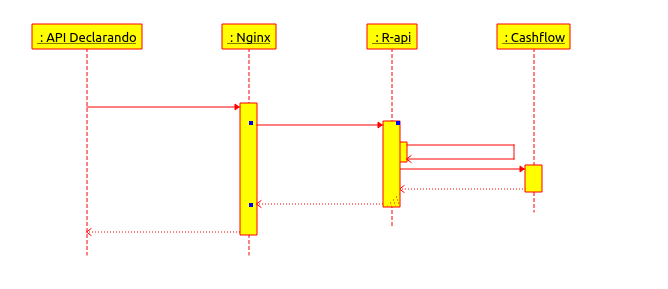
\includegraphics[width=1\textwidth]{20210407_1_estructura_clases.png}
%    \label{fig:estructura_clases}
%  \end{figure}
%\end{frame}


\end{document}
